\chapter*{前言}

\vfill
\begin{center}

    \arm{\ait {\Large اُطْلُبُوْا العِلْمَ وَلَوْ في الصِّينِ.}}
    
    ~\\

    \emph{求知,哪怕在中国。}
\end{center}
\vfill

\begin{center}
    \begin{center}
        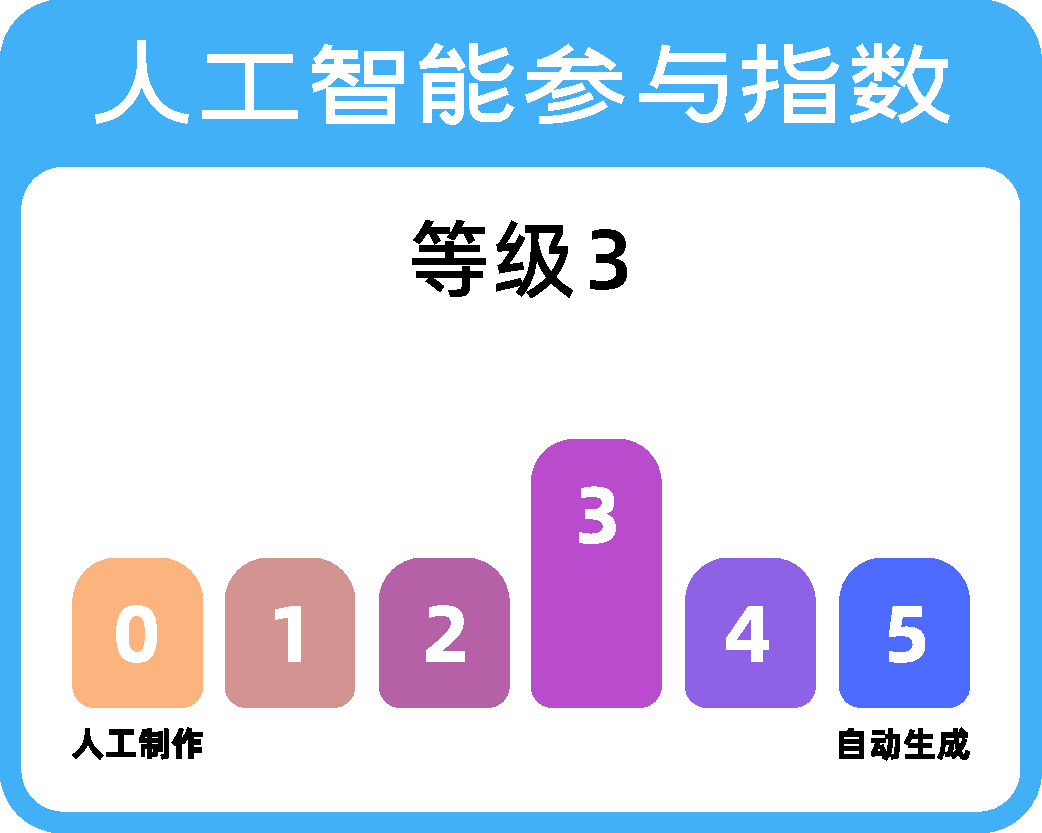
\includegraphics[width=0.4\textwidth]{img/iiia.pdf}
    \end{center}
\end{center}

本笔记借助了GitHub Copilot生成。这玩意太好用了,甚至能猜想到例句(不过发音符号有时会标错),我审核了AI生成的所有内容,但由于毕竟是新接触一套书写系统,难免有拼写疏漏。

\begin{attention}
    这样的格式代表老师在课上强调的知识点。
\end{attention}

\begin{note}
    这样的格式代表我自己的感悟。
\end{note}